\section{Numerical Setup and Results}

In this Section we first introduce the experimental setup used to produce the
results, and then discuss the actual results. The results here act both as a
proof of principle of the data space estimators presented in this paper but also
as part of a suite of methodological validation tools, see also the "future
tests" \cite{Cruz_Martinez_2021}, used to understand the PDF uncertainties of
the upcoming NNPDF4.0 set of PDFs. For the purpose of understanding how the
results here were produced, we will briefly describe the key features of the
NNPDF4.0 methodology, but refer the reader to NNPDF4.0 for a full discussion on
how these methodological choices were made, and the impact on performing PDF
fits to experimental data.

\subsection{Neural network parton distribution functions}

Using neural networks to fit PDFs has been discussed many times in previous
NNPDF publications, see for example \cite{nnpdf30, Ball_2017}. A new feature of
NNPDF4.0 will be that, for the default fit performed in the evolution basis, a
single neural network parameterises all 8 PDF flavours $\{ g, \Sigma, V, V_3,
V_8, T_3, T_8, c^+ \}$ at the initial scale. The PDF for a single flavour $j$,
at the initial scale $Q_0 = 1.65~{\rm GeV}$ is given by
\begin{equation}
    f_j(x, Q_0) = NN(x, \ln x | \modelvec)_j * x^{1-\alpha_j} * (1-x)^{\beta_j},
\end{equation}
where $\alpha$ and $\beta$ are the preprocessing exponents, which control the
PDF behaviour at $x \to 0$ and $x \to 1$ respectively and $NN(x, \ln x |
\modelvec)_j$ is the $j^{\rm th}$ output of the neural network, which takes $x$
and $\ln x$ as input. As discussed in Sec.~\ref{sec:fit-reps}, an ensemble of
models is fitted, each one is an MAP estimator of the corresponding pseudo-data
it is fitted on. Unlike in the case of the linear model, the parameters of the
neural network cannot be found analytically and instead an optimization
algorithm is used to try and find the parameters which maximise the likelihood.
In principle, the preprocessing exponents can also be varied during the fit
analogously to the neural network parameters, such as in \cite{Carrazza_2019},
or they can be randomly selected from a predetermined range as is done in
previous NNPDF releases, for example \cite{Ball_2017}. There are clearly many
choices with respect to hyperparameters, the discussion of how these choices
have been made is beyond the scope of this paper and left to the full NNPDF4.0
release \cite{NNPDF40}. A summary of the hyperparameters used to produce results
presented in this paper are provided in Tab.~\ref{tab:Hyperparams}.

Finally, the parton distributions themselves are not compared directly with
data. Instead the observables quantities are obtained by performing convolutions
with the PDFs, as discussed in \ref{eq:DISExample}. In practice the observables
are obtained by convoluting the PDFs with FastKernel tables, presented in
\cite{Ball_2010,Bertone_2017}, for each data point. The convolution depends on
the process type of the observable, for DIS-like observables, such as in
Eq.~\ref{eq:DISExample}, the convolution is performed with a single PDF. For
hadronic observables the convolution is performed between two PDFs.

\subsection{Closure test setup}

As input to the closure test, a single replica was drawn randomly from a
previous NNPDF fit to experimental data. We refer to this as the underlying law
and the corresponding predictions the true observable values. An example of the
gluon input is provided in Fig.~\ref{fig:InputGluonPDF}. In principle any
function could be used as underlying law, however it makes sense to use a
realistic input.

\begin{figure}
    \centering
    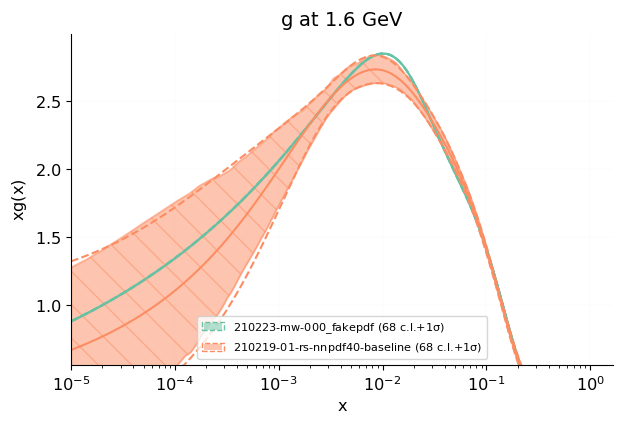
\includegraphics[width=0.8 \textwidth]{plot_pdfs_g.png}
    \caption{The green line is the input underlying law for the gluon PDF,
    which is sampled from the ensemble from a fit to data. The 68\% confidence
    interval is plotted for those replicas as the orange band.}
    \label{fig:InputGluonPDF}
\end{figure}

The observables used in the fits are a subset of the full NNPDF4.0 dataset. For
convenience, we chose to fit the PDFs on a variant of the NNPDF3.1 dataset used
in Ref.~\cite{Ball_2018}, which is described in detail in a study of the
determination of the strange PDF~\cite{Faura_2020}. The datasets used in the
calculation of statistical estimators are the new datasets which will be
included in NNPDF4.0, which will be discussed in detail with the main release.
For a full summary of observables used in the test data and a visual
representation of the kinematic region of both the training and testing data,
see App.~\ref{sec:appendix-datasets}.

The choice of data for both fitting and testing is considered unimportant, one
could consider splitting the data into training and test in a way which
considered kinematic coverage rather than this naive chronological splitting.
Alternatively, since the data is generated from the theory predictions produced
by the input underlying law, one could even produce completely artificial data
using a different set of FK tables. From a practical standpoint, using the
NNPDF3.1 dataset and validating on the newly included datasets in 4.0 allowed us
to validate the PDF uncertainities on data outside of the kinematic coverage of
data included in the fit. Furthermore, the data estimators only give us local
information on the PDF uncertainties and it seems logical to split the data in
this way since the results seem more applicable to the reality of how the PDFs
end up being used.

We then generate 30 different sets of experimental central values (or L1 data),
as discussed in Sec.~\ref{sec:closure-test-intro}, for the fitted 3.1-like
dataset. Each set of experimental central values was then fitted following
NNPDF4.0 methodology \cite{NNPDF40}, producing 40 pseudo-data replicas.

When comparing with the old NNPDF methodology, we use the minimization algorithm
of Ref.~\cite{nnpdf30}. An important iingredient of previous NNPDF minimization
procedure was the choice of a stopping criterion. XXX

\subsection{Errors on PDFs}

The relative error on fitted PDFs is shown in Fig.~\ref{fig:nnpdfLfits}.

\begin{figure}[ht]
    \centering
    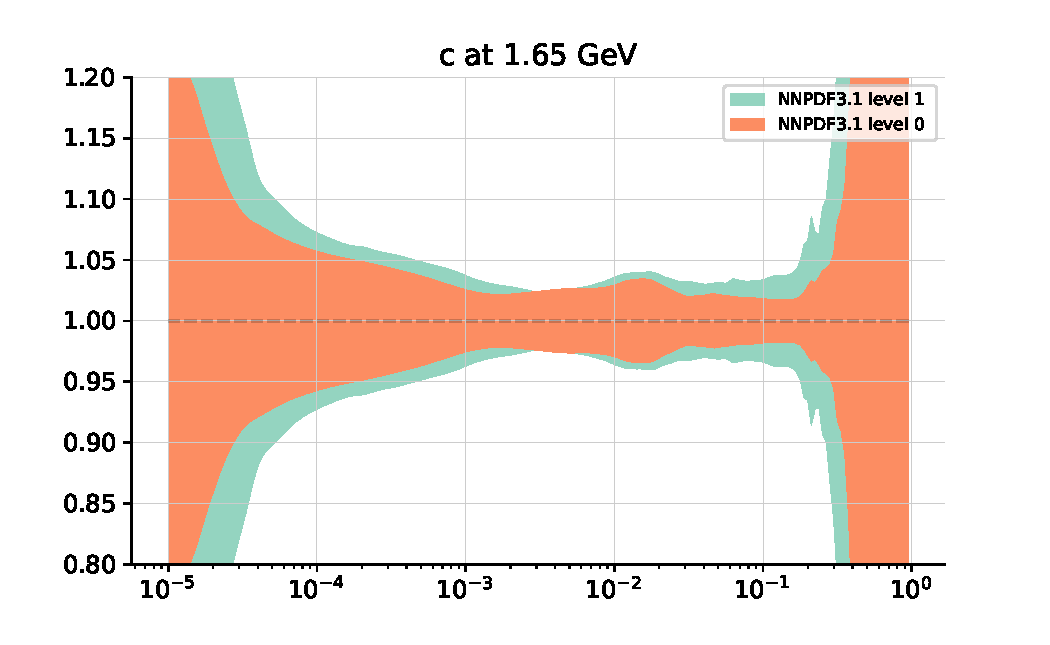
\includegraphics[scale=0.7]{CT_log_c_nnpdf31_L0_L1.pdf}
    \caption{Relative error in nnfit clsoure tests.}
    \label{fig:nnpdfLfits}    
\end{figure}

\subsection{Bias-variance ratio}

We calculated $\biasvarratio$ on the test data, shown in
Tab.~\ref{tab:summarise_new_data}. An
uncertainty on $\biasvarratio$ by performing a bootstrap sample
\cite{efron1994introduction},
where we randomly sample from both fits and replicas and re-calculate
$\biasvarratio$, the value and error presented in the table is then the mean
and standard deviation across bootstrap samples. We checked that the distribution
of the estimator across bootstrap samples is indeed Gaussian. We also checked
that increasing the number of fits and replicas reduced the bootstrap error but
the central values were the same within the estimated bootstrap uncertainities.

\begin{table}[hb]
    \begin{center}
        \begin{tabular}{lr}
            \toprule
            {}     &  $\biasvarratio$ \\
            \midrule
            Total  &  $1.03\pm0.05$   \\
            \bottomrule
            \end{tabular}
    \end{center}
    \caption{
        The bias-variance ratio, $\biasvarratio$, for unseen data, summarised in
        Tab.~\ref{tab:summarise_new_data}. The uncertainty is estimated by
        performing a bootstrap sample across fits and replicas and calculating
        the standard deviation. We see that overall $\biasvarratio$ is consistent
        with 1, within uncertainities. This gives a good indication that, at least
        for the unseen data used in this study, the uncertainities are faithful.
    }
    \label{tab:biasvarratio}
\end{table}

One can also compare qualitatively the distribution of bias across fits, to the
distribution of the difference between replica predictions and expectation
values of predictions (in units of the covariance) across different fits
and replicas. The square root ratio of the mean of these two distributions
is precisely $\biasvarratio$.

\begin{figure}[ht]
    \centering
    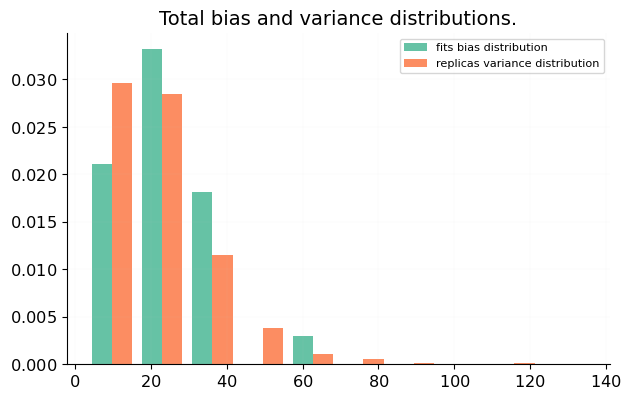
\includegraphics[width=0.8 \textwidth]{plot_bias_variance_distributions_total.png}
    \caption{The green histogram is the distribution of the total bias across fits,
    the orange histogram is the distribution of the difference between the
    replica and central predictions squared, in units of the covariance
    across all fits and replicas. This gives a qualitative picture of the full
    distribution, in Tab.~\ref{tab:biasvarratio} we compare the square root of the
    mean of each distribution.}
\end{figure}

\subsection{Comparison to quantile statistics}

As discussed in Sec.~\ref{sec:QuantileStatistics}, one can define an analogous
estimator in data space, based upon $\xi_{n\sigma}$, which was defined on a grid
of points in $x$ and $Q^2$ in PDF space in \cite{nnpdf30}. There is not
a one-to-one correspondence
between this and $\biasvarratio$, but a loose approximation using
Eq.~\ref{eq:expectedxi}. In Tab.~\ref{tab:xicomparison} we compare the estimated
$\xi_{1\sigma}$ from
subsituting $\biasvarratio$ into Eq.~\ref{eq:expectedxi} and to the
measured value.

\begin{table}[hb]
    \begin{center}
        \begin{tabular}{lrr}
            \toprule
            {}     & $\xi_{1\sigma}$ & $\erf(\biasvarratio/\sqrt{2})$ \\
            \midrule
            Total  & $0.69\pm0.02$   & $0.67\pm0.03$                  \\
            \bottomrule
            \end{tabular}
    \end{center}
    \caption{
        Comparing the measured value of $\xi_1\sigma$ and the estimated
        value from $\biasvarratio$. The two values are consistent, which
        suggests the approximation that the ratio of uncertainties is
        approximately the same across all data is not completely invalidated.
        Not only are the measured value and estimated value from $\biasvarratio$
        self consistent, but they are also consistent with $0.68$, which
        further supports the argument that the model uncertainities are
        faithful.
    }
    \label{tab:xicomparison}
\end{table}

Despite the assumptions entering each of the two estimators differing, we see
good agreement between the $\xi_{1\sigma}$ estimated from $\biasvarratio$
and that measured directly. We find this result reassuring, since it indicates
not only that the total uncertainty averaged across all data is faithful, but
also that the uncertainty on each data point seems faithful. If the results
differed it would indicate some kind of imbalance, where some components
of the uncertainty are correctly represented by the replicas but other directions
are not.
